\subsection{Image classification} \label{sec:mnist}

Our first example features an LBDN trained to classify the MNIST dataset \cite{LeCun++2010}. We will use this example to demonstrate how training image classifiers with LBDNs makes them robust to adversarial attacks thanks to the built-in Lipschitz bound. For a detailed investigation of the effect of Lipschitz bounds on classification robustness and reliability, please see \cite{Wang+Manchester2023}.

% Load the data
\subsubsection{Load the data} \label{sec:mnist-data}

We begin by loading the training and test data. \verb|MLDatasets.jl|\footnote{\url{https://juliaml.github.io/MLDatasets.jl/}} contains a number of common machine-learning datasets, including the MNIST dataset. To load the full dataset of 60,000 training images and 10,000 test images, one would run the following code.

\begin{lstlisting}[language = Julia]
using MLDatasets: MNIST

T = Float32
x_train, y_train = MNIST(T, split=:train)[:]
x_test,  y_test  = MNIST(T, split=:test)[:]
\end{lstlisting}

The feature matrices \verb|x_train| and \verb|x_test| are three-dimensional arrays where each 28x28 layer contains pixel data for a single handwritten number from 0 to 9 (eg: see Fig. \ref{fig:mnist_numbers}). The labels \verb|y_train| and \verb|y_test| are vectors containing the classification of each image as a number from 0 to 9. We convert each of these to a format better suited to training with \verb|Flux.jl|.

\begin{lstlisting}[language = Julia]
using Flux

# Reshape features for model input
x_train = Flux.flatten(x_train)
x_test  = Flux.flatten(x_test)

# Encode categorical outputs and store
y_train = Flux.onehotbatch(y_train, 0:9)
y_test  = Flux.onehotbatch(y_test,  0:9)
data = [(x_train, y_train)]
\end{lstlisting}

Features are now stored in a $28^2\times N$ \verb|Matrix| where each column contains pixel data from a single image, and the labels have been converted to a $10\times N$ \verb|Flux.OneHotMatrix| where each column contains a 1 in the row corresponding to the image's classification (eg: row 3 for an image showing the number 2) and a 0 otherwise.

% Define a model
\subsubsection{Define a model} \label{sec:mnist-model}

We can now construct an LBDN model to train on the MNIST dataset. The larger the model, the better the classification accuracy will be, at the cost of longer training times. The smaller the Lipschitz bound $\gamma$, the more robust the model will be to input perturbations (such as noise in the image). If $\gamma$ is too small, however, it can restrict the model flexibility and limit the achievable performance \cite{Wang+Manchester2023}. For this example, we use a small network of two 64-neuron hidden layers and set a Lipschitz bound of $\gamma=5.0$ just to demonstrate the method.

\begin{lstlisting}[language = Julia]
using RobustNeuralNetworks

# Model specification
nu = 28*28              # Inputs (size of image)
ny = 10                 # Outputs (classifications)
nh = fill(64,2)         # Hidden layers 
γ  = 5.0f0              # Lipschitz bound 5.0

# Define parameters,create model
model_ps = DenseLBDNParams{T}(nu, nh, ny, γ)
model = Chain(DiffLBDN(model_ps), Flux.softmax)
\end{lstlisting}

The \verb|model| consists of two parts. The first is a callable \verb|DiffLBDN| model constructed from its direct parameterization, which is defined by an instance of \verb|DenseLBDNParams| as per Section \ref{sec:parameterizations}. The output is then converted to a probability distribution using a \verb|softmax| layer. Note that all \verb|AbstractLBDN| models can be combined with traditional neural network layers using \verb|Flux.Chain|. 

We could also have constructed the \verb|model| from a combination of \verb|SandwichFC| layers. Introduced in \cite{Wang+Manchester2023}, the \verb|SandwichFC| layer is a fully-connected or dense layer with a guaranteed Lipschitz bound of 1.0. We have designed the user interface for \verb|SandwichFC| to be as similar to that of \verb|Flux.Dense| as possible.
\begin{lstlisting}[language = Julia]
model = Chain(
    (x) -> (sqrt(γ) * x),
    SandwichFC(nu => nh[1], relu; T),
    SandwichFC(nh[1] => nh[2], relu; T),
    (x) -> (sqrt(γ) * x),
    SandwichFC(nh[2] => ny; output_layer=true, T),
    Flux.softmax
)
\end{lstlisting}
This model is equivalent to a dense LBDN constructed with \verb|LBDN| or \verb|DiffLBDN|. We have included it as a convenience for users familiar with layer-wise network construction in \verb|Flux.jl|, and recommend using it interchangeably with \verb|DiffLBDN|.

% Define a loss function
\subsubsection{Define a loss function} \label{sec:mnist-loss}

A typical loss function for training on datasets with discrete labels is the cross entropy loss. We can use the \verb|crossentropy| loss function shipped with \verb|Flux.jl|.

\begin{lstlisting}[language = Julia]
loss(model,x,y) = Flux.crossentropy(model(x), y)
\end{lstlisting}

% Train the model
\subsubsection{Train the model} \label{sec:mnist-train}

We train the model over 600 epochs using two learning rates: \verb|1e-3| for the first 300, and \verb|1e-4| for the last 300. We use the \verb|Adam| optimizer \cite{Kingma+Ba2015} and the default \verb|Flux.train!| method for convenience. Note that the \verb|Flux.train!| method updates the learnable parameters each time the model is evaluated on a batch of data, hence our choice of \verb|DiffLBDN| as a model wrapper.

\begin{lstlisting}[language = Julia]
# Hyperparameters
epochs = 300
lrs = [1e-3,1e-4]

# Train with the Adam optimizer
for k in eachindex(lrs)
    opt_state = Flux.setup(Adam(lrs[k]), model)
    for i in 1:epochs
        Flux.train!(loss, model, data, opt_state)
    end
end
\end{lstlisting}

% Evaluate the trained model
\subsubsection{Evaluate the trained model} \label{sec:mnist-evaluate}

Our final model achieves training and test accuracies of approximately 99\% and 98\%, respectively, as shown in Table \ref{tab:mnist-results}. We could improve this further by switching to a convolutional LBDN, as in \cite{Wang+Manchester2023}. Some examples of classifications given by the trained LBDN model are presented in Figure \ref{fig:mnist_numbers}.

\begin{figure}[!t]
    \centering
    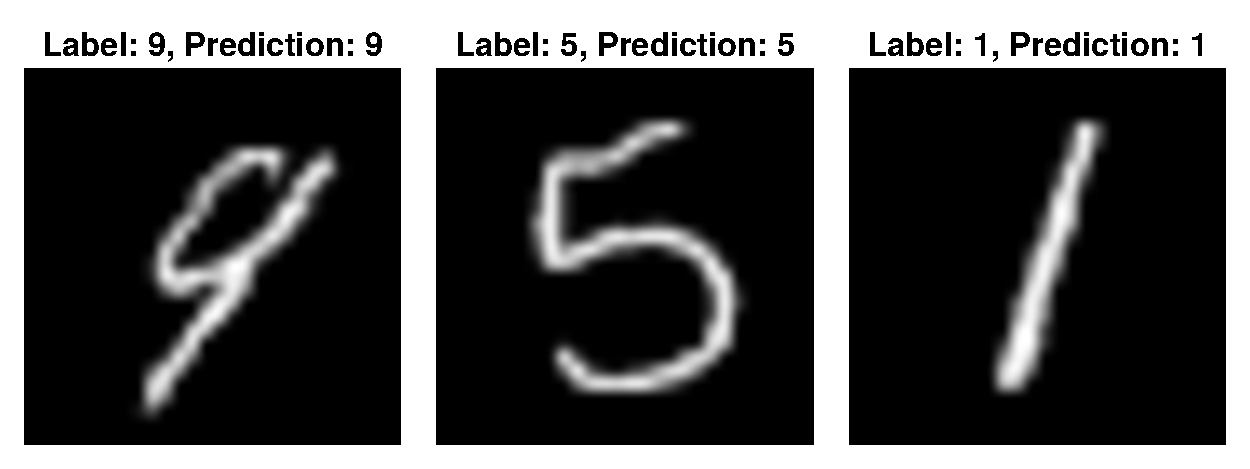
\includegraphics[width=0.47\textwidth]{Images/lbdn_mnist.pdf}
    \caption{Examples of classifications from the trained LBDN model on the MNIST dataset.}
    \label{fig:mnist_numbers}
\end{figure}

% Investigate robustness
\subsubsection{Investigate robustness} \label{sec:mnist-robustness}

The main advantage of using an LBDN for image classification is its built-in robustness to noise (or attacks) added to the image. This robustness is a direct benefit of the Lipschitz bound. As outlined in the Section \ref{sec:robustness-lipschitz}, the Lipschitz bound effectively defines how ``smooth'' the network is: the smaller the Lipschitz bound, the less the network outputs will change as the inputs vary. For example, small amounts of noise added to the image will be less likely to change its classification. A detailed investigation into this effect is presented in \cite{Wang+Manchester2023}.

We can demonstrate the robustness of LBDNs by comparing the model to a standard MLP built from \verb|Flux.Dense| layers. We first create a \verb|dense| network with the same layer structure as the LBDN.
\begin{lstlisting}[language = Julia]
# Initialisation functions
init = Flux.glorot_normal
initb(n) = Flux.glorot_normal(n)

# Build a dense model
dense = Chain(
    Dense(nu, nh[1], relu; 
          init, bias=initb(nh[1])),
    Dense(nh[1], nh[2], relu; 
          init, bias=initb(nh[2])),
    Dense(nh[2], ny; init, bias=initb(ny)),
    Flux.softmax
)
\end{lstlisting}

Training the \verb|dense| model with the same training loop used for the LBDN model results in a model that achieves training and test accuracies of approximately 98\% and 97\%, respectively, as shown in Table \ref{tab:mnist-results}.

\begin{table} [ht]
\tbl{Training and test accuracy for the LBDN and Dense models on the MNIST dataset without perturbations.}{
\begin{tabular}{|l|c|c|}\hline
    \textbf{Model structure} & \textbf{Training accuracy (\%)} & \textbf{Test accuracy (\%)} \\ \hline
    LBDN & 98.7 & 97.6 \\ \hline
    Dense & 98.4 & 96.9 \\ \hline
\end{tabular}}
\label{tab:mnist-results}
\end{table}

As a simple test of robustness, we add uniformly-sampled random noise in the range $[-\epsilon, \epsilon]$ to the pixel data in the test dataset for a range of noise magnitudes $\epsilon \in [0, 200/255].$ We record the test accuracy for each perturbation size and store it for plotting.
\begin{lstlisting}[language = Julia]
using Statistics

# Get test accuracy as we add noise
uniform(x) = 2*rand(T, size(x)...) .- 1
compare(y, yh) = 
    maximum(yh, dims=1) .== maximum(y.*yh, dims=1)
accuracy(model, x, y) = mean(compare(y, model(x)))
    
function noisy_test_error(model, ϵ)
    noisy_xtest = x_test .+ ϵ*uniform(x_test)
    accuracy(model, noisy_xtest,  y_test)*100
end

ϵs = T.(LinRange(0, 200, 10)) ./ 255
lbdn_error  = noisy_test_error.((model,), ϵs)
dense_error = noisy_test_error.((dense,), ϵs)
\end{lstlisting}

Plotting the results in Figure \ref{fig:mnist_robust} very clearly shows that the \verb|dense| network, which has no guarantees on its Lipschitz bound, quickly loses its accuracy as small amounts of noise are added to the image. In contrast, the LBDN \verb|model| maintains its accuracy even when the (maximum) perturbation size is as much as 80\% of the maximum pixel values. This is an illustration of why image classification is one of the most promising use-cases for LBDN models. For a more detailed comparison of LBDN with state-of-the-art image classification methods, see \cite{Wang+Manchester2023}.

\begin{figure}[!b]
    \centering
    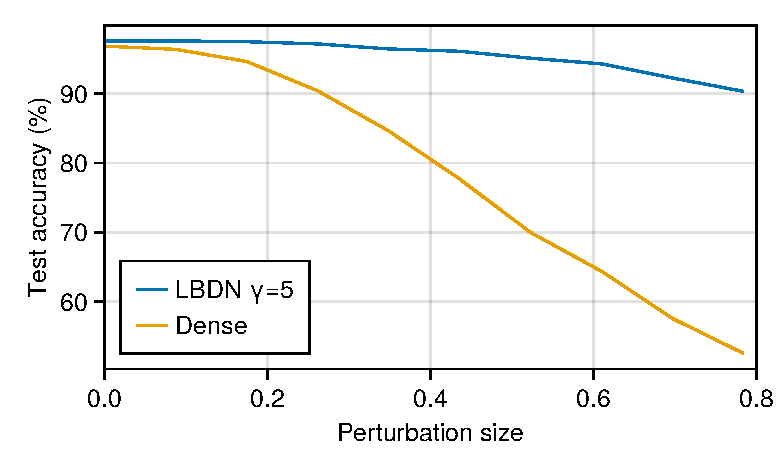
\includegraphics[width=0.47\textwidth]{Images/lbdn_mnist_robust.pdf}
    \caption{Comparison of test accuracy on the MNIST dataset as a function of random perturbation magnitude $\epsilon$. The LBDN model is significantly more robust than a standard \texttt{Dense} network.}
    \label{fig:mnist_robust}
\end{figure}
